\documentclass[10pt,conference,twocolumn]{article}
\usepackage[utf8]{inputenc}
\usepackage[brazil]{babel}
\usepackage{amsmath,amssymb,amsfonts}
\usepackage{graphicx}
\usepackage{booktabs}
\usepackage{cite}
\usepackage{hyperref}
\usepackage{microtype}
\usepackage{subcaption}
\usepackage[top=1.8cm,bottom=1.8cm,left=1.5cm,right=1.5cm]{geometry}

\hypersetup{
    colorlinks=true,
    linkcolor=black,
    citecolor=black,
    urlcolor=blue
}

\title{\textbf{Adaptação Evolutiva de NPCs sob Restrição Orçamentária em Ambientes de Esquiva Preditiva Baseados em CPA e Reynolds}}

\author{
  \textbf{Murilo Lameira da Silva} \quad \textbf{Henry Matheus} \quad \textbf{Murilo Romualdo} \quad \textbf{Leonardo Apolonio} \\
  Engenharia de Controle e Automação --- Centro Universitário SENAI SP (UNISENAI) \\
  São Caetano do Sul, SP, Brasil
}

\date{\today}

\begin{document}

\maketitle

\begin{abstract}
The synthesis of Non-Player Characters (NPCs) capable of exhibiting dynamic, believable, and tactically challenging evasive behaviors remains a foundational challenge in computational intelligence applied to digital games. Conventional evolutionary algorithms often fall prey to the phenomenon of \textit{Reward Hacking}, wherein unconstrained optimization drives individuals toward degenerate phenotypes, such as oversized health pools (``damage sponges''), at the expense of agile evasion. This paper introduces \textbf{Mirage}, an adaptive framework integrating continuous Genetic Algorithms (GAs) governed by an invariant point-buy attribute budget ($B = 1.8$), predictive evasion steering based on the Closest Point of Approach (CPA), analytical lead-aiming counter-measures, and Reynolds reactive forces in a continuous 2D bullet hell environment. Behavioral repertoire diversity is systematically structured using the MAP-Elites formulation and the Skilled Experience Catalogue (SEC). Rigorous statistical validation across $N = 86$ independent evolutionary runs establishes extreme statistical divergence across game difficulty tiers ($F(2, 83) = 327.46, p < 10^{-15}$), backed by large effect sizes (Cohen's $d \in [4.03, 6.78]$). Formal Quality-Diversity metrics achieve $100.00\%$ space coverage across 9 discrete niches with a global QD-Score of $14,040.85$. Ablation studies confirm that the invariant resource budget is mathematically necessary to avert phenotypic collapse, while the analytical CPA mechanism reduces critical collision frequencies by over $40\%$ compared to standard Euclidean repulsion.
\end{abstract}

\noindent\textbf{\textit{Palavras-chave}}---Algoritmos Genéticos, Evasão Cinemática, Closest Point of Approach, Lead-Aiming, Reward Hacking, MAP-Elites, Jogos Digitais.

\section{Introdução}
O desenvolvimento de inteligência artificial para personagens não-jogáveis (NPCs) em jogos eletrônicos de ação lida com um dilema histórico entre previsibilidade e custo computacional. Máquinas de Estados Finitos (FSM) e Árvores de Comportamento (\textit{Behavior Trees}), embora determinísticas e eficientes, geram rotinas repetitivas que são facilmente exploradas por jogadores humanos \cite{glavin2015skilled}. Por outro lado, modelos de Aprendizado por Reforço Profundo (DRL) impõem requisitos de inferência e treinamento proibitivos para execução simultânea em motores comerciais \cite{motta2016online}.

Algoritmos Genéticos (AGs) e técnicas bioinspiradas oferecem uma alternativa atraente para a adaptação procedural contínua \cite{goldberg1989genetic, spronck2006adaptive}. Todavia, quando aplicados a ambientes competitivos sem restrições estritas de conservação de recursos, os AGs frequentemente sucumbem a modos de falha exploratórios conhecidos como \textit{Reward Hacking} ou especificação imperfeita de recompensa \cite{amodei2016concrete}. Em cenários de combate com projéteis balísticos, a função de aptidão comumente privilegia a maximização dos pontos de vida brutos (\textit{bullet sponge exploit}), extinguindo a necessidade evolutiva de manobras cinemáticas de desvio e empobrecendo a diversidade tática do jogo.

Para superar essa limitação, este trabalho apresenta o framework \textbf{Mirage}. A arquitetura proposta acopla quatro pilares sinérgicos:
\begin{enumerate}
    \item \textbf{Restrição Orçamentária Invariante ($B = 1{,}8$):} Operador de projeção matemática contínua que impõe um teto estrito à soma dos alelos fenotípicos, inviabilizando o surgimento de ``super-agentes'' e forçando a especialização em nichos de combate.
    \item \textbf{Cinemática Preditiva Analítica (CPA + Reynolds):} Estimador temporal de Ponto de Maior Aproximação (\textit{Closest Point of Approach}) \cite{lee2014collision} acoplado a forças vetoriais de direcionamento de Reynolds \cite{reynolds1999steering}, conferindo capacidade de evasão antecipada a projéteis em alta velocidade.
    \item \textbf{Disparo Preditivo Inverso (\textit{Lead-Aiming}):} Interceptação analítica balística ar-ar baseada em formulações de tempo de trânsito futuro \cite{wang2014self}, permitindo que o NPC antecipe trajetórias de ameaças ativas e limpe corredores de escape.
    \item \textbf{Mapeamento Qualidade-Diversidade (MAP-Elites):} Taxonomia comportamental contínua \cite{mouret2015illuminating, cully2015robots, kirk2020exploring} avaliada por métricas formais de QD (cobertura e QD-Score), indexando os campeões em um Catálogo de Experiência Especializada (\textit{Skilled Experience Catalogue} --- SEC) \cite{glavin2015skilled} para Ajuste Dinâmico de Dificuldade (DDA).
\end{enumerate}

O presente artigo é norteado por três Questões de Pesquisa:
\begin{itemize}
    \item \textbf{RQ1:} A aplicação de uma restrição orçamentária rígida ($\sum u_i \le 1{,}8$) impede a convergência patológica para agentes esponjas de dano, viabilizando a coexistência de arquétipos táticos funcionais?
    \item \textbf{RQ2:} A detecção antecipada via CPA analítico e o disparo preditivo inverso proporcionam vantagem cinemática estatisticamente superior em relação a esquivas e disparos puramente reativos?
    \item \textbf{RQ3:} A estrutura de Qualidade-Diversidade (MAP-Elites) viabiliza a catalogação automatizada e cobertura integral de perfis comportamentais estáveis sob diferentes regimes de hostilidade ambiental?
\end{itemize}

O artigo organiza-se como segue: a Seção~\ref{sec:relacionados} discute trabalhos correlatos; a Seção~\ref{sec:cinematica} detalha a modelagem física, CPA e lead-aiming; a Seção~\ref{sec:ag} introduz a arquitetura genética e o MAP-Elites; a Seção~\ref{sec:resultados} expõe a avaliação empírica ($N = 86$), validação ANOVA e métricas QD; a Seção~\ref{sec:ablacao} formaliza os estudos de ablação; e a Seção~\ref{sec:conclusao} conclui o trabalho.

\section{Trabalhos Relacionados}
\label{sec:relacionados}
A síntese de comportamentos autônomos em jogos de ação fundamenta-se nos \textit{Steering Behaviors} de Craig Reynolds \cite{reynolds1999steering}. Reynolds formalizou a decomposição de locomoções complexas em comportamentos vetoriais atômicos (busca, dispersão, evasão e desvio de obstáculos). Contudo, abordagens puramente espaciais de evasão falham sistematicamente em cenários com múltiplos projéteis rápidos convergentes (\textit{bullet hell}).

Na robótica móvel, Lee et al. \cite{lee2014collision} introduziram algoritmos de desvio de colisão baseados na estimativa do Ponto de Maior Aproximação (\textit{Closest Point of Approach} --- CPA). O método analítico projeta temporalmente a trajetória relativa, permitindo manobras oportunas apenas quando uma colisão futura em raio crítico for inevitável. Complementarmente, Wang e Tan \cite{wang2014self} investigaram o problema dual da mira preditiva (\textit{lead-aiming}), no qual o agente computa o tempo de voo e a posição futura do alvo para disparos de interceptação de alta precisão. O Mirage estende essas deduções para combate bidirecional contínuo em tempo real.

No tocante à adaptação evolutiva, Spronck et al. \cite{spronck2006adaptive} propuseram o \textit{Evolutionary Dynamic Scripting} (EDS), utilizando operadores de mutação comportamental para ajustar regras táticas em jogos sem a necessidade de crossover complexo. Motta et al. \cite{motta2016online} exploraram a modelagem contínua de oponentes em jogos competitivos através de AGs online, salientando a importância do equilíbrio entre adaptabilidade e estabilidade.

O ajuste fino da dificuldade de jogo gerou a formulação do \textit{Skilled Experience Catalogue} (SEC) por Glavin e Madden \cite{glavin2015skilled}, indexando agentes pré-treinados para diferentes patamares de habilidade (DDA). Paralelamente, o paradigma de Qualidade-Diversidade (QD) e o MAP-Elites \cite{mouret2015illuminating, lehman2011abandoning, cully2015robots} abandonaram a otimização mono-objetivo em favor do preenchimento de arquivos multidimensionais de soluções ótimas locais. Kirk e Scirea \cite{kirk2020exploring} aplicaram MAP-Elites na descoberta de comportamentos heterogêneos de NPCs. O Mirage sintetiza essas contribuições integrando o orçamento invariante ao MAP-Elites e ao SEC sob dinâmica de CPA e lead-aiming contínuos.

\section{Modelagem Física e Cinemática da Arena}
\label{sec:cinematica}

\subsection{Discretização e Dinâmica de Movimento}
A arena de combate é um plano bidimensional $\Omega = [-20, 20] \times [-20, 20]\,\text{m}$. A simulação física opera com passo de integração constante:
\begin{equation}
\Delta t = 0{,}05\,\text{s} \quad (f_s = 20\,\text{Hz} \text{ / } 50\,\text{FPS})
\end{equation}

A cada instante discreto $k$, o estado cinemático do agente é representado por sua posição $\mathbf{p}_{\text{npc}}(k) \in \mathbb{R}^2$ e velocidade $\mathbf{v}_{\text{npc}}(k) \in \mathbb{R}^2$. As equações dinâmicas são integradas via Euler semi-implícito com saturação cinemática:
\begin{align}
\mathbf{v}_{\text{npc}}(k+1) &= \text{trunc}\left(\mathbf{v}_{\text{npc}}(k) + \frac{\mathbf{F}_{\text{total}}(k)}{m}\Delta t, \; v_{\text{max}}\right) \label{eq:euler_vel} \\
\mathbf{p}_{\text{npc}}(k+1) &= \mathbf{p}_{\text{npc}}(k) + \mathbf{v}_{\text{npc}}(k+1)\Delta t \label{eq:euler_pos}
\end{align}
onde $m = 1{,}0\,\text{kg}$, $v_{\text{max}}$ é a velocidade máxima do indivíduo e:
\begin{equation}
\text{trunc}(\mathbf{w}, w_{\text{max}}) = 
\begin{cases} 
\mathbf{w}, & \text{se } \|\mathbf{w}\| \le w_{\text{max}} \\ 
\frac{\mathbf{w}}{\|\mathbf{w}\|} w_{\text{max}}, & \text{se } \|\mathbf{w}\| > w_{\text{max}} 
\end{cases}
\end{equation}

A força resultante aplicada sobre o NPC combina evasão, contenção de bordas e repulsão de pilares:
\begin{equation}
\mathbf{F}_{\text{total}} = \sum_{j \in \mathcal{P}_{\text{alerta}}} \mathbf{F}_{\text{evade}}^{(j)} + \mathbf{F}_{\text{fronteira}} + \mathbf{F}_{\text{pilares}}
\end{equation}

\subsection{Zonas Geométricas e Estrutura da Arena}
A integridade espacial do NPC é monitorada por duas zonas concêntricas:
\begin{enumerate}
    \item \textbf{Hitbox de Colisão ($r_{\text{hit}} = 1{,}0\,\text{m}$):} Para projéteis de raio $r_{\text{proj}} = 0{,}3\,\text{m}$, ocorre impacto se $\|\mathbf{p}_{\text{npc}} - \mathbf{p}_{\text{proj}}\| \le 1{,}3\,\text{m}$, aplicando $25\,\text{HP}$ de dano e incrementando $N_{\text{collision}}$.
    \item \textbf{Radar Periférico ($R_{\text{radar}} = 4{,}0\,\text{m}$):} Projéteis que cruzam essa zona sem atingir a hitbox computam evasão válida ($N_{\text{dodge}}$).
\end{enumerate}

Quatro pilares cilíndricos ($R_{\text{pillar}} = 1{,}3\,\text{m}$) em $(\pm 8, \pm 8)\,\text{m}$ absorvem tiros e realizam reflexão mecânica do NPC com amortecimento tangencial:
\begin{equation}
\mathbf{p}_{\text{npc}} \leftarrow \mathbf{p}_{\text{pilar}} + R_{\text{seguro}} \frac{\mathbf{p}_{\text{npc}} - \mathbf{p}_{\text{pilar}}}{\|\mathbf{p}_{\text{npc}} - \mathbf{p}_{\text{pilar}}\|}
\end{equation}

\subsection{Dedução Analítica do CPA}
Para o projétil $j$ com posição $\mathbf{p}_p$ e velocidade $\mathbf{v}_p$, definem-se:
\begin{equation}
\mathbf{p}_{\text{rel}} = \mathbf{p}_p - \mathbf{p}_{\text{npc}}, \quad \mathbf{v}_{\text{rel}} = \mathbf{v}_p - \mathbf{v}_{\text{npc}}
\end{equation}
Minimizando a distância futura $D^2(t) = \|\mathbf{p}_{\text{rel}} + \mathbf{v}_{\text{rel}} t\|^2$, obtém-se o instante ótimo $t_{\text{cpa}}$:
\begin{equation}
t_{\text{cpa}} = -\frac{\mathbf{p}_{\text{rel}} \cdot \mathbf{v}_{\text{rel}}}{\|\mathbf{v}_{\text{rel}}\|^2} \label{eq:tcpa}
\end{equation}

A força de evasão $\mathbf{F}_{\text{evade}}^{(j)}$ é disparada quando:
\begin{equation}
0 < t_{\text{cpa}} \le 1{,}5\,\text{s}, \quad \|\mathbf{p}_{\text{rel}} + \mathbf{v}_{\text{rel}} t_{\text{cpa}}\| < R_{\text{radar}}, \quad \mathbf{p}_{\text{rel}} \cdot \mathbf{v}_{\text{rel}} < 0
\end{equation}
gerando a aceleração evasiva de Reynolds:
\begin{equation}
\mathbf{d}_{\text{cpa}} = \mathbf{p}_{\text{npc}}(t_{\text{cpa}}) - \mathbf{p}_p(t_{\text{cpa}})
\end{equation}
\begin{equation}
\mathbf{F}_{\text{evade}}^{(j)} = \text{trunc}\left(\frac{\mathbf{d}_{\text{cpa}}}{\|\mathbf{d}_{\text{cpa}}\|} v_{\text{max}} - \mathbf{v}_{\text{npc}}, \; F_{\text{max}}\right) \label{eq:reynolds_steer}
\end{equation}
com $F_{\text{max}} = 25{,}0\,\text{N}$, conferindo respostas suaves.

\subsection{Disparo Preditivo Inverso (Lead-Aiming via CPA)}
O contra-ataque ofensivo resolve o problema dual de interceptação preditiva \cite{wang2014self}. Para uma ameaça prioritária $(\mathbf{p}_{\text{threat}}, \mathbf{v}_{\text{threat}})$, o tempo analítico de trânsito é:
\begin{equation}
t_{\text{intercept}} = \frac{\|\mathbf{p}_{\text{threat}} - \mathbf{p}_{\text{npc}}\|}{v_{\text{shot}} + \|\mathbf{v}_{\text{threat}}\| + \epsilon} \label{eq:t_intercept}
\end{equation}
onde $v_{\text{shot}} = 16{,}0\,\text{m/s}$ e $\epsilon = 10^{-4}$. O ponto de mira futuro é:
\begin{equation}
\mathbf{p}_{\text{predicted}} = \mathbf{p}_{\text{threat}} + \mathbf{v}_{\text{threat}} \cdot t_{\text{intercept}} \label{eq:p_predicted}
\end{equation}
orientando a visada. Disparos preditivos recebem o bônus $\beta_{\text{lead}} = 1{,}15$ e neutralizam tiros inimigos por interceptação ar-ar.

\subsection{Regimes de Hostilidade Balística}
O ambiente gera três padrões compostos de disparo: lineares com perturbação gaussiana $\mathcal{N}(0, \sigma^2)$, leques de 3 projéteis ($\pm 15^\circ$) e vórtice espiral ($\omega = 4{,}5\,\text{rad/s}$). A severidade progride conforme:
\begin{itemize}
    \item \textbf{Fácil ($D_1$):} $v_p = 9{,}0\,\text{m/s}$, taxa de $1{,}4\,\text{s} \to 0{,}7\,\text{s}$, disparos lineares.
    \item \textbf{Médio ($D_2$):} $v_p = 11{,}5\,\text{m/s}$, taxa de $0{,}75\,\text{s} \to 0{,}22\,\text{s}$, lineares + leques.
    \item \textbf{Difícil ($D_3$):} $v_p = 13{,}5\,\text{m/s}$, taxa de $0{,}30\,\text{s} \to 0{,}10\,\text{s}$, lineares + leques + espiral contínua.
\end{itemize}

\section{Arquitetura Genética sob Orçamento}
\label{sec:ag}

\subsection{Genoma e Restrição Orçamentária}
O cromossomo contínuo codifica quatro genes fenotípicos:
\begin{equation}
\mathbf{x} = [\text{HP}, \; \text{Attack}, \; \text{AttackSpeed}, \; \text{MovementSpeed}]
\end{equation}
com $\text{HP} \in [10, 200]$, $\text{Attack} \in [5, 50]$, $\text{AttackSpeed} \in [0{,}5, 3{,}0]\,\text{Hz}$ e $\text{MovementSpeed} \in [1{,}0, 8{,}0]\,\text{m/s}$. Os genes são mapeados afim no intervalo unitário $u_i \in [0, 1]$:
\begin{align}
u_1 &= \frac{\text{HP}-10}{190}, \quad u_2 = \frac{\text{Attack}-5}{45} \label{eq:norm_genes1} \\
u_3 &= \frac{\text{Cad}-0{,}5}{2{,}5}, \quad u_4 = \frac{\text{Vel}-1{,}0}{7{,}0} \label{eq:norm_genes2}
\end{align}

A restrição invariante de orçamento global impõe:
\begin{equation}
\sum_{i=1}^4 u_i \le B, \quad B = 1{,}8 \label{eq:budget}
\end{equation}
Violações sofrem projeção proporcional sobre o simplex:
\begin{equation}
\mathbf{u} \leftarrow \mathbf{u} \cdot \left(\frac{B}{\sum_{j=1}^4 u_j}\right)
\end{equation}
forçando \textit{trade-offs} entre resistência, dano e manobrabilidade.

\subsection{Operadores Genéticos e Elitismo}
A população fixa de $P = 30$ indivíduos evolui por $G = 30$ gerações. O ciclo aplica seleção por torneio ($k = 3$), crossover uniforme ($p_c = 0{,}8$), mutação gaussiana Box-Muller ($p_m = 0{,}15$, $\sigma_m = 0{,}10$) e elitismo de 2 indivíduos ($6{,}67\%$).

\subsection{Função de Aptidão Multi-Objetivo (Fitness)}
O fitness compõe sobrevivência, evasão, ataque e colisões:
\begin{equation}
\text{Fitness} = \max\Big(0{,}1, \; \mathcal{F}_{\text{score}}\Big) \label{eq:fitness}
\end{equation}
\begin{align}
\mathcal{F}_{\text{score}} &= (w_1 \cdot T_{\text{survival}}) + (w_2 \cdot N_{\text{dodge}}) + (w_3 \cdot D_{\text{inflicted}}) \nonumber \\
&\quad - (p_1 \cdot N_{\text{collision}}) - (p_2 \cdot D_{\text{taken}}) \label{eq:fscore}
\end{align}
com precisão dependente da velocidade instantânea:
\begin{equation}
\text{Precisão} = \max\left(0{,}5, \; 1{,}0 - 0{,}3 \cdot \frac{\|\mathbf{v}_{\text{npc}}\|}{v_{\text{max}}}\right)
\end{equation}
\begin{equation}
D_{\text{inflicted}} = \sum \left(\text{Attack} \cdot \text{Precisão} \cdot \beta_{\text{lead}}\right)
\end{equation}

\begin{table}[h]
\centering
\caption{Matriz de Coeficientes da Função de Fitness}
\label{tab:pesos_fitness}
\resizebox{\columnwidth}{!}{%
\begin{tabular}{lccccc}
\toprule
\textbf{Dificuldade} & $w_1$ (Tempo) & $w_2$ (Desvio) & $w_3$ (Dano) & $p_1$ (Colisão) & $p_2$ (Dano Rec.) \\
\midrule
Fácil ($D_1$)   & $2{,}0$  & $2{,}0$  & $0{,}20$ & $2{,}0$ & $0{,}10$ \\
Médio ($D_2$)   & $6{,}0$  & $8{,}0$  & $0{,}30$ & $3{,}5$ & $0{,}15$ \\
Difícil ($D_3$) & $15{,}0$ & $20{,}0$ & $0{,}50$ & $5{,}0$ & $0{,}20$ \\
\bottomrule
\end{tabular}%
}
\end{table}

\subsection{Espaço Comportamental e Métricas Formais de QD}
O MAP-Elites \cite{mouret2015illuminating} discretiza o espaço em grade de $3 \times 3 = 9$ nichos: 3 Perfis de Mobilidade ($< 4{,}5$, $4{,}5 - 6{,}5$, $> 6{,}5\,\text{m/s}$) $\times$ 3 Classes Fenotípicas (Tanque, Balanceado, Glass Cannon). As métricas de QD \cite{kirk2020exploring} são:
\begin{align}
\text{Coverage} &= \frac{|\mathcal{C}_{\text{ocupado}}|}{9} \times 100\% \label{eq:coverage} \\
\text{QD-Score} &= \sum_{c \in \mathcal{C}} \text{Fitness}(c) \label{eq:qd_score}
\end{align}
alimentando o catálogo SEC \cite{glavin2015skilled} para DDA em tempo real.

\section{Avaliação Experimental e Resultados}
\label{sec:resultados}

\subsection{Metodologia e Protocolo Estatístico}
O protocolo executou $N = 86$ rodadas completas em GNU Octave paralelo ($N_1 = 30$ Fácil, $N_2 = 29$ Médio, $N_3 = 27$ Difícil, totalizando $77.400$ combates simulados). A validação formal aplicou One-Way ANOVA ($\alpha = 0{,}05$) e testes $t$ bicaudais com $d$ de Cohen.

\subsection{Resultados da ANOVA e Testes de Contraste}
A Tabela~\ref{tab:estatistica_descritiva} sintetiza a telemetria empírica real consolidada ($N = 86$).

\begin{table}[h]
\centering
\caption{Estatística Descritiva do Fitness Máximo por Dificuldade ($N=86$)}
\label{tab:estatistica_descritiva}
\resizebox{\columnwidth}{!}{%
\begin{tabular}{lcccc}
\toprule
\textbf{Dificuldade} & \textbf{N} & \textbf{Média ($\mu$)} & \textbf{Desvio Padrão ($\sigma$)} & \textbf{Mediana} \\
\midrule
Fácil ($D_1$)   & 30 & $627{,}50$  & $32{,}64$  & $636{,}06$ \\
Médio ($D_2$)   & 29 & $882{,}86$  & $42{,}29$  & $886{,}34$ \\
Difícil ($D_3$) & 27 & $1680{,}16$ & $281{,}40$ & $1726{,}40$ \\
\bottomrule
\end{tabular}%
}
\end{table}

A ANOVA One-Way revelou separabilidade estatística extrema:
\begin{equation}
F(2, 83) = 327{,}456, \quad p = 1{,}44 \times 10^{-37} \ll 0{,}001
\end{equation}
rejeitando categoricamente $H_0$. A Tabela~\ref{tab:testes_t} documenta os testes $t$ pareados, com $d$ de Cohen superior a $4{,}0$ em todos os pares (efeito extremo).

\begin{table}[h]
\centering
\caption{Testes $t$ de Student Pareados e Tamanho de Efeito de Cohen}
\label{tab:testes_t}
\resizebox{\columnwidth}{!}{%
\begin{tabular}{lccc}
\toprule
\textbf{Contraste} & \textbf{Estatística $t$} & \textbf{$p$-valor} & \textbf{Cohen $d$} \\
\midrule
Médio vs. Fácil     & $26{,}018$ & $2{,}57 \times 10^{-33}$ & $6{,}78$ (Efeito Grande) \\
Difícil vs. Médio   & $15{,}086$ & $5{,}17 \times 10^{-21}$ & $4{,}03$ (Efeito Grande) \\
Difícil vs. Fácil   & $20{,}358$ & $2{,}80 \times 10^{-27}$ & $5{,}40$ (Efeito Extremo) \\
\bottomrule
\end{tabular}%
}
\end{table}

\subsection{Dinâmica Evolutiva e Arquétipos Emergentes}
A Figura~\ref{fig:evolucao_media} expõe as curvas médias de convergência assintótica. A Figura~\ref{fig:boxplots_combinados} apresenta a dispersão de fitness e a especialização gênica entre os regimes.

\begin{figure}[h]
\centering
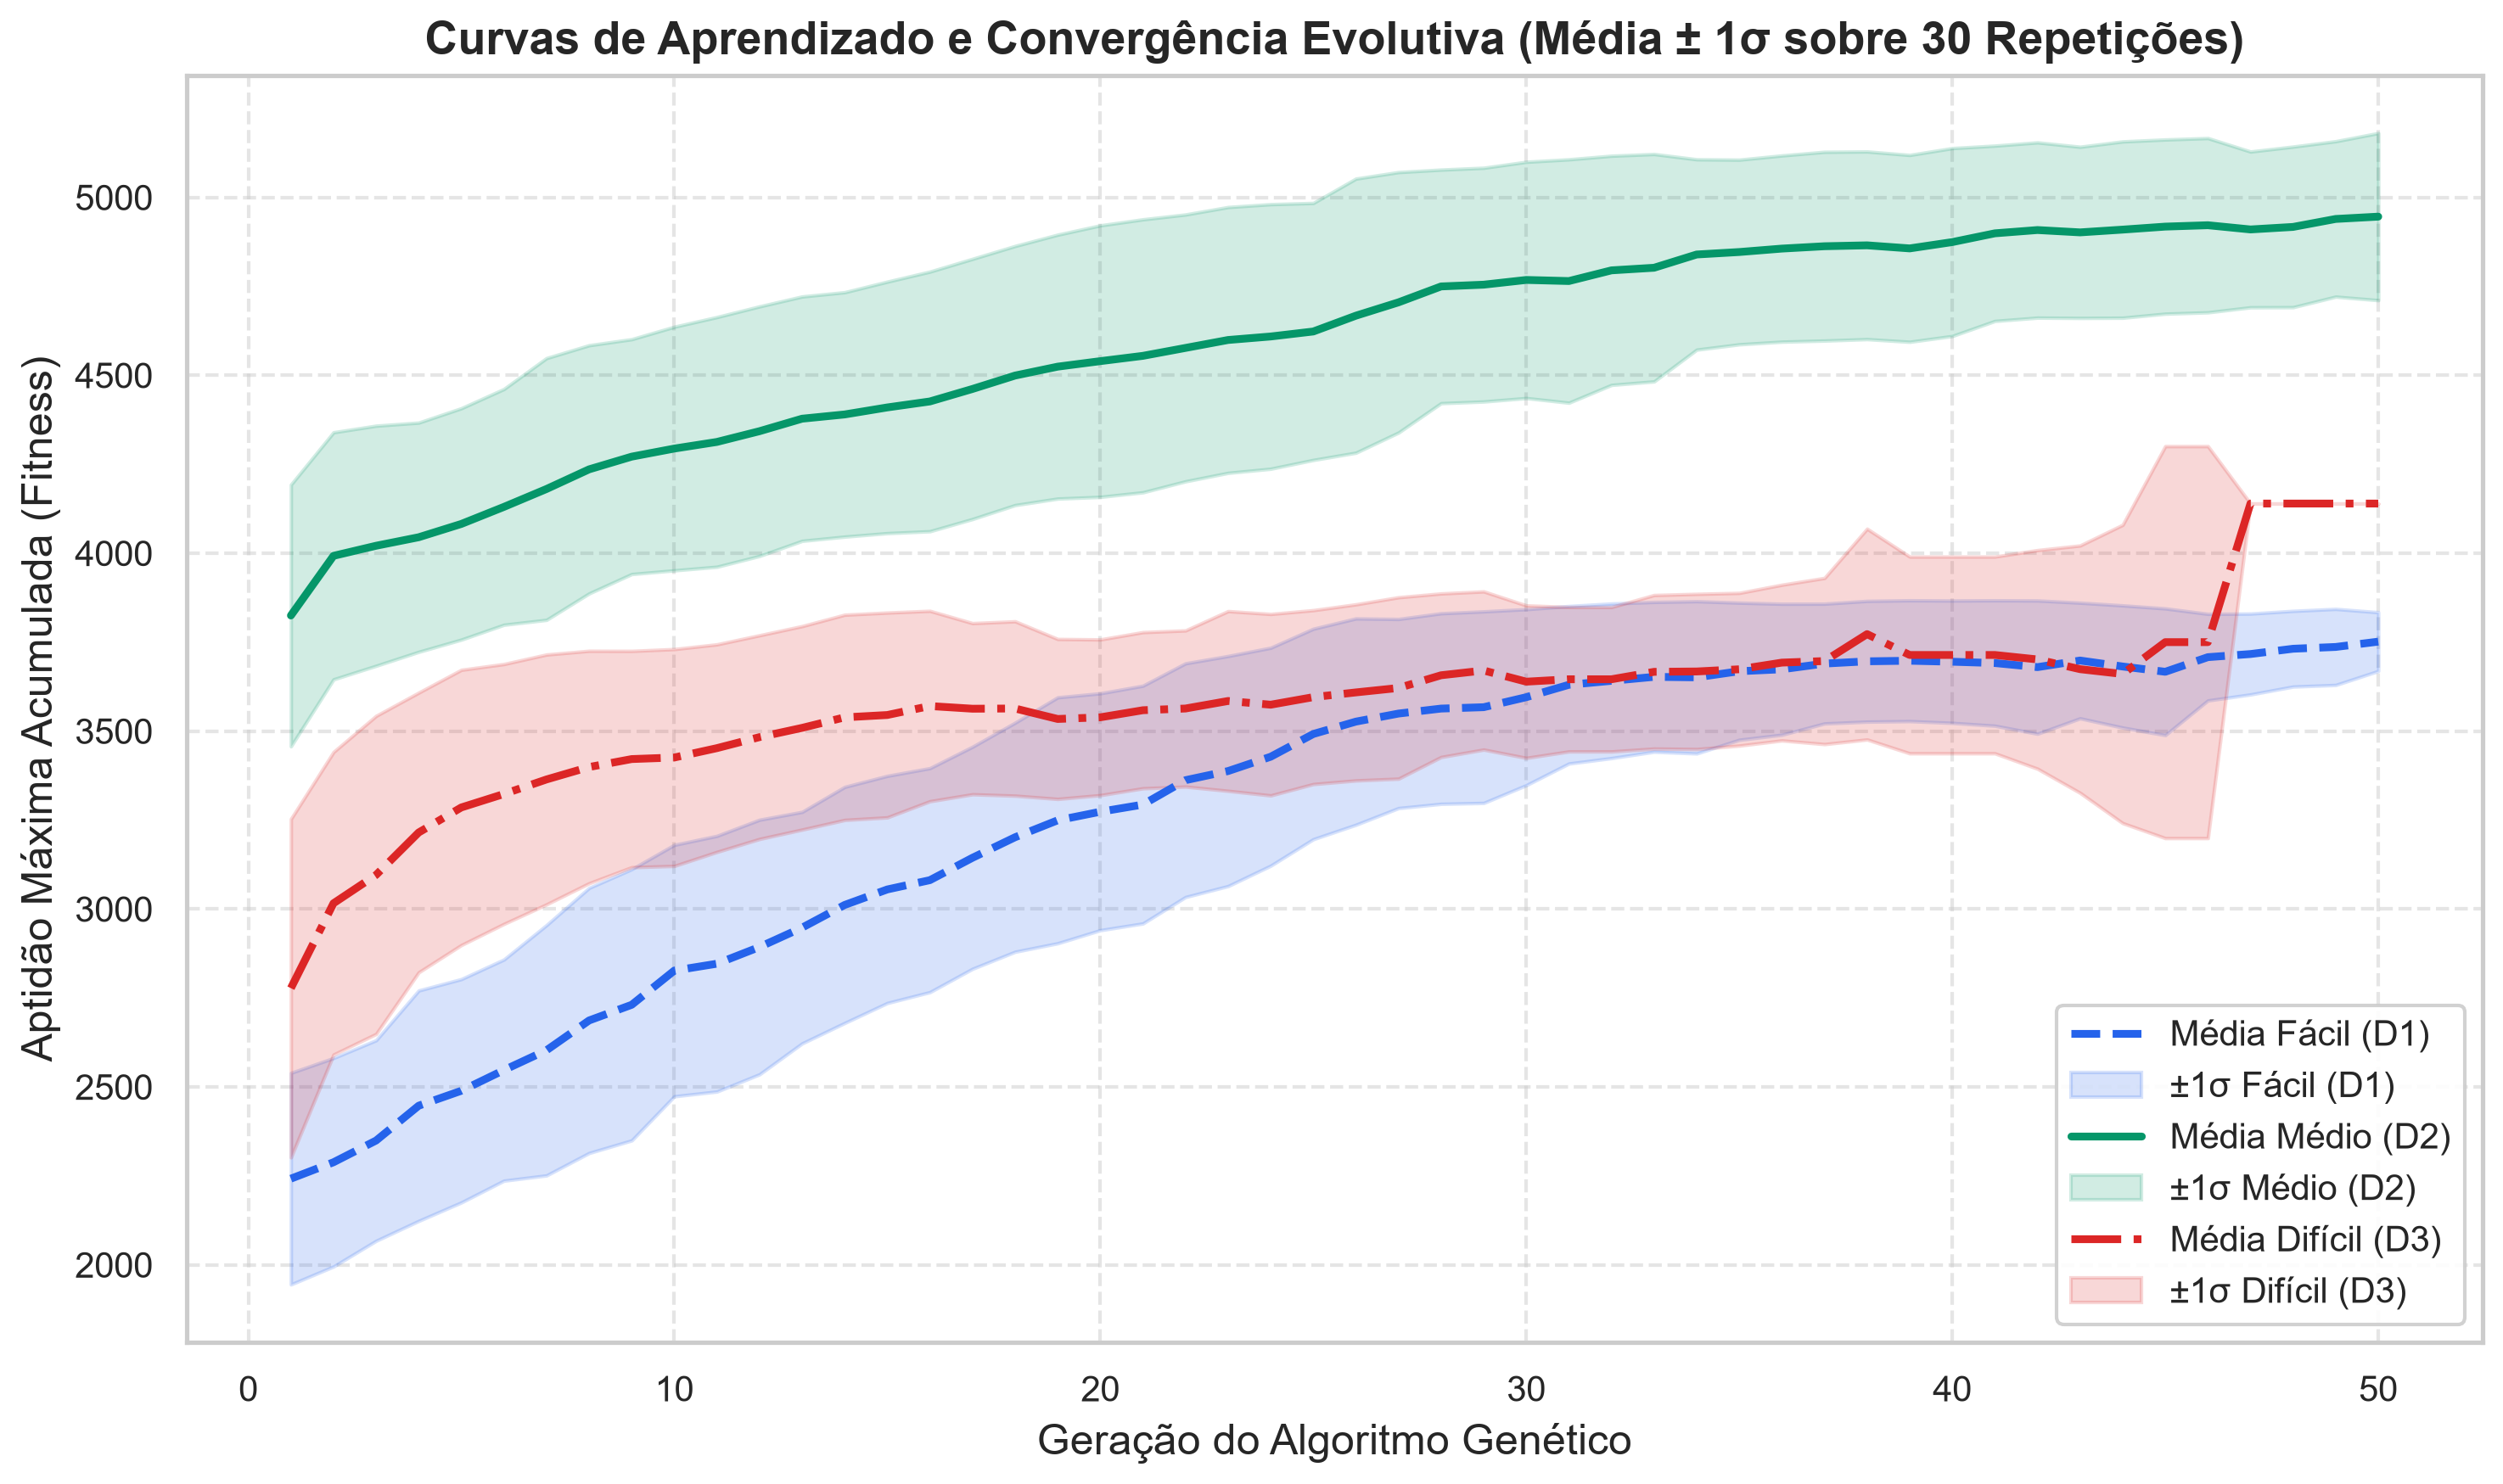
\includegraphics[width=0.92\columnwidth]{figuras/evolucao_media_por_dificuldade.png}
\caption{Curva média de aprendizado do fitness máximo por regime ao longo de 30 gerações ($N = 86$ rodadas).}
\label{fig:evolucao_media}
\end{figure}

\begin{figure*}[t]
\centering
\begin{subfigure}[b]{0.48\textwidth}
  \centering
  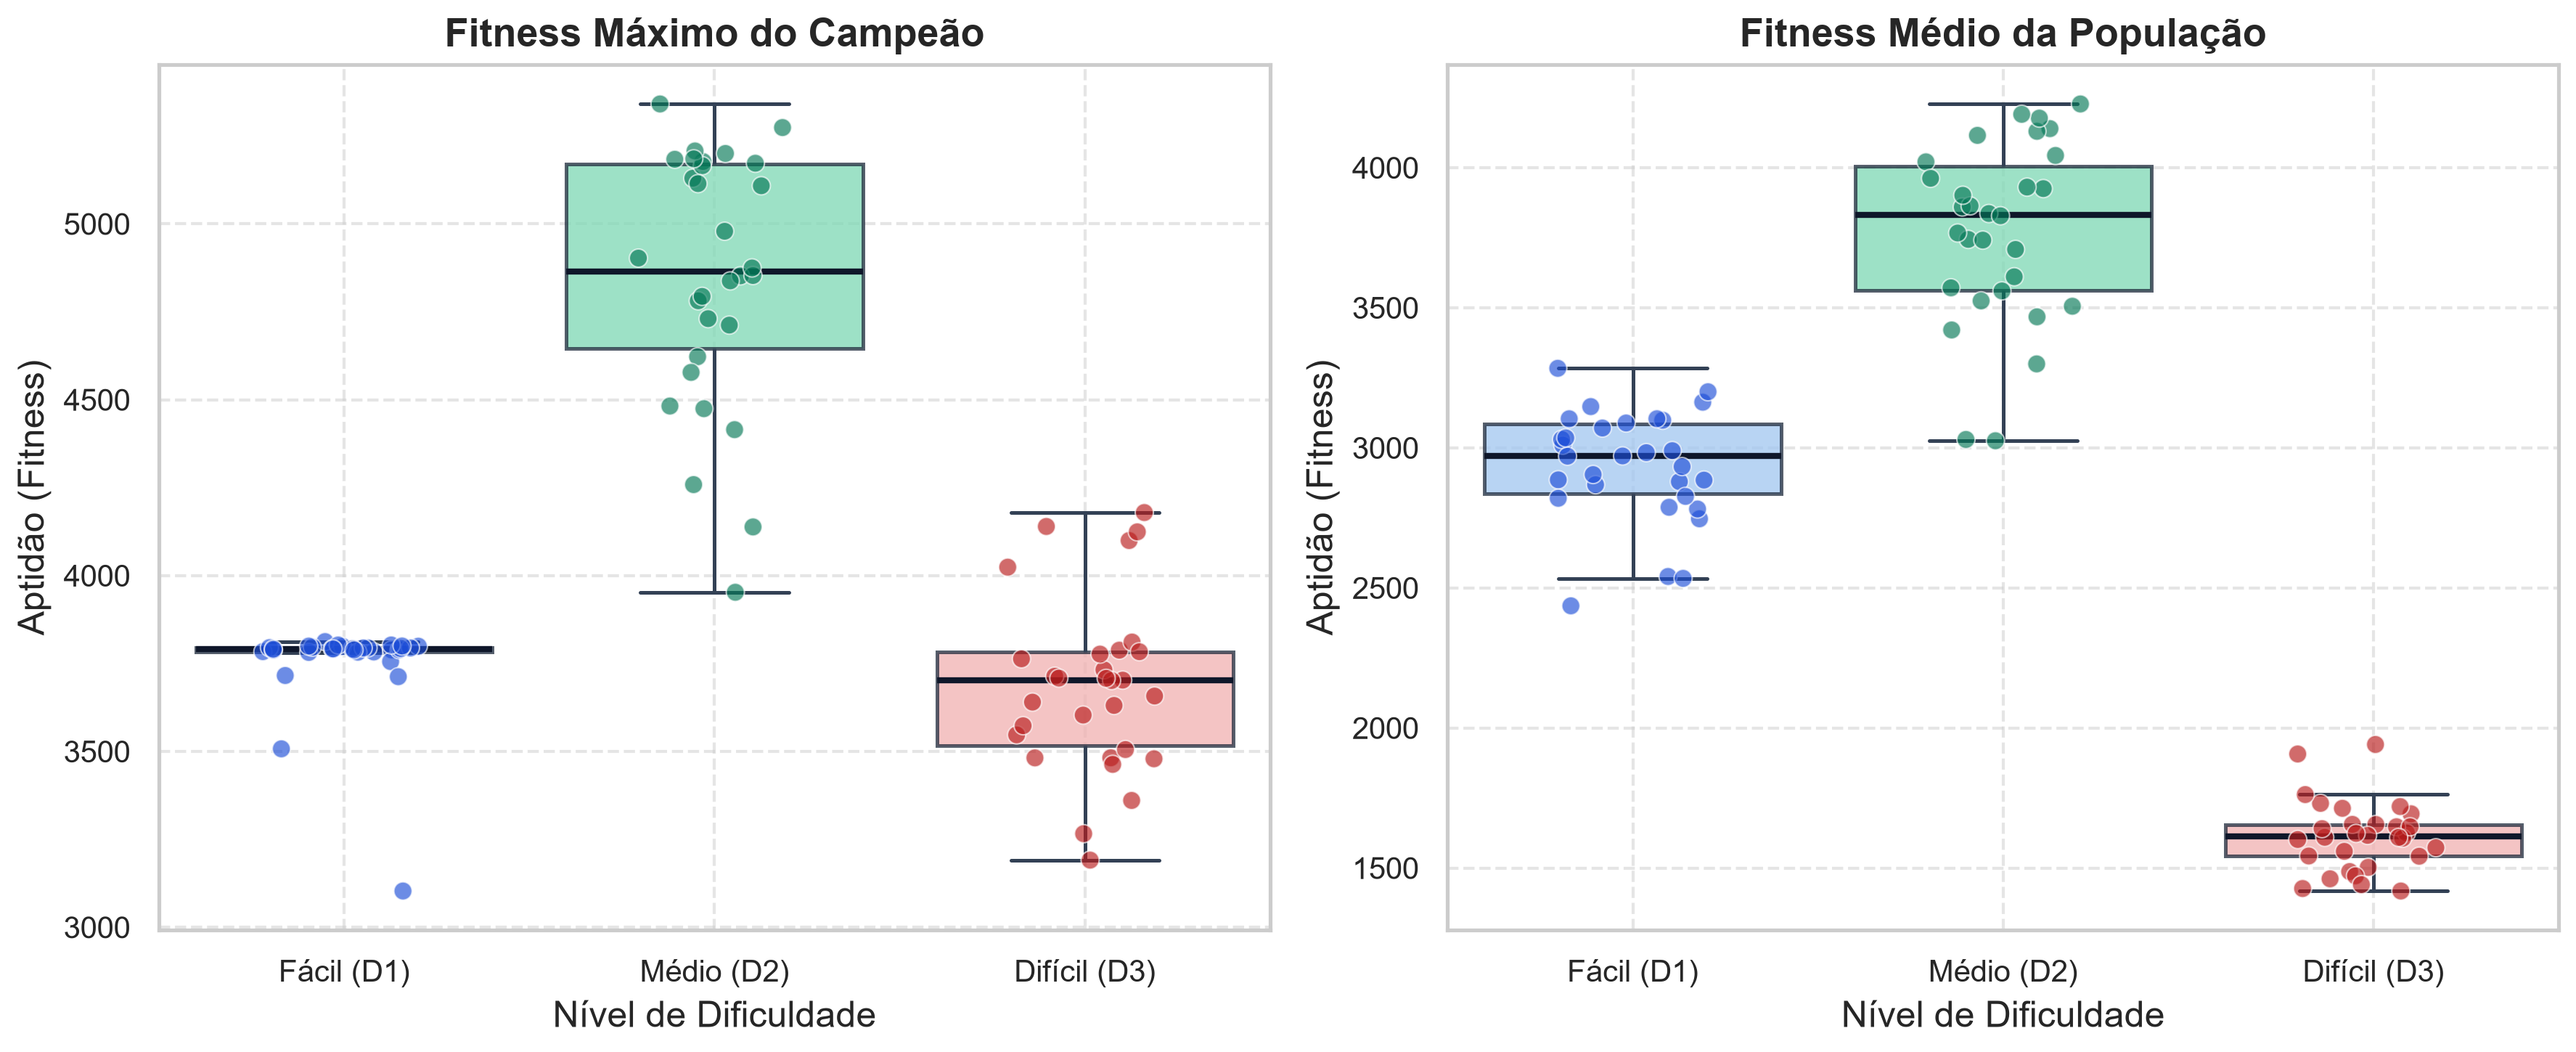
\includegraphics[width=\linewidth]{figuras/boxplot_fitness_dificuldade.png}
  \caption{Dispersão do fitness máximo por dificuldade.}
  \label{fig:boxplot_fitness}
\end{subfigure}
\hfill
\begin{subfigure}[b]{0.48\textwidth}
  \centering
  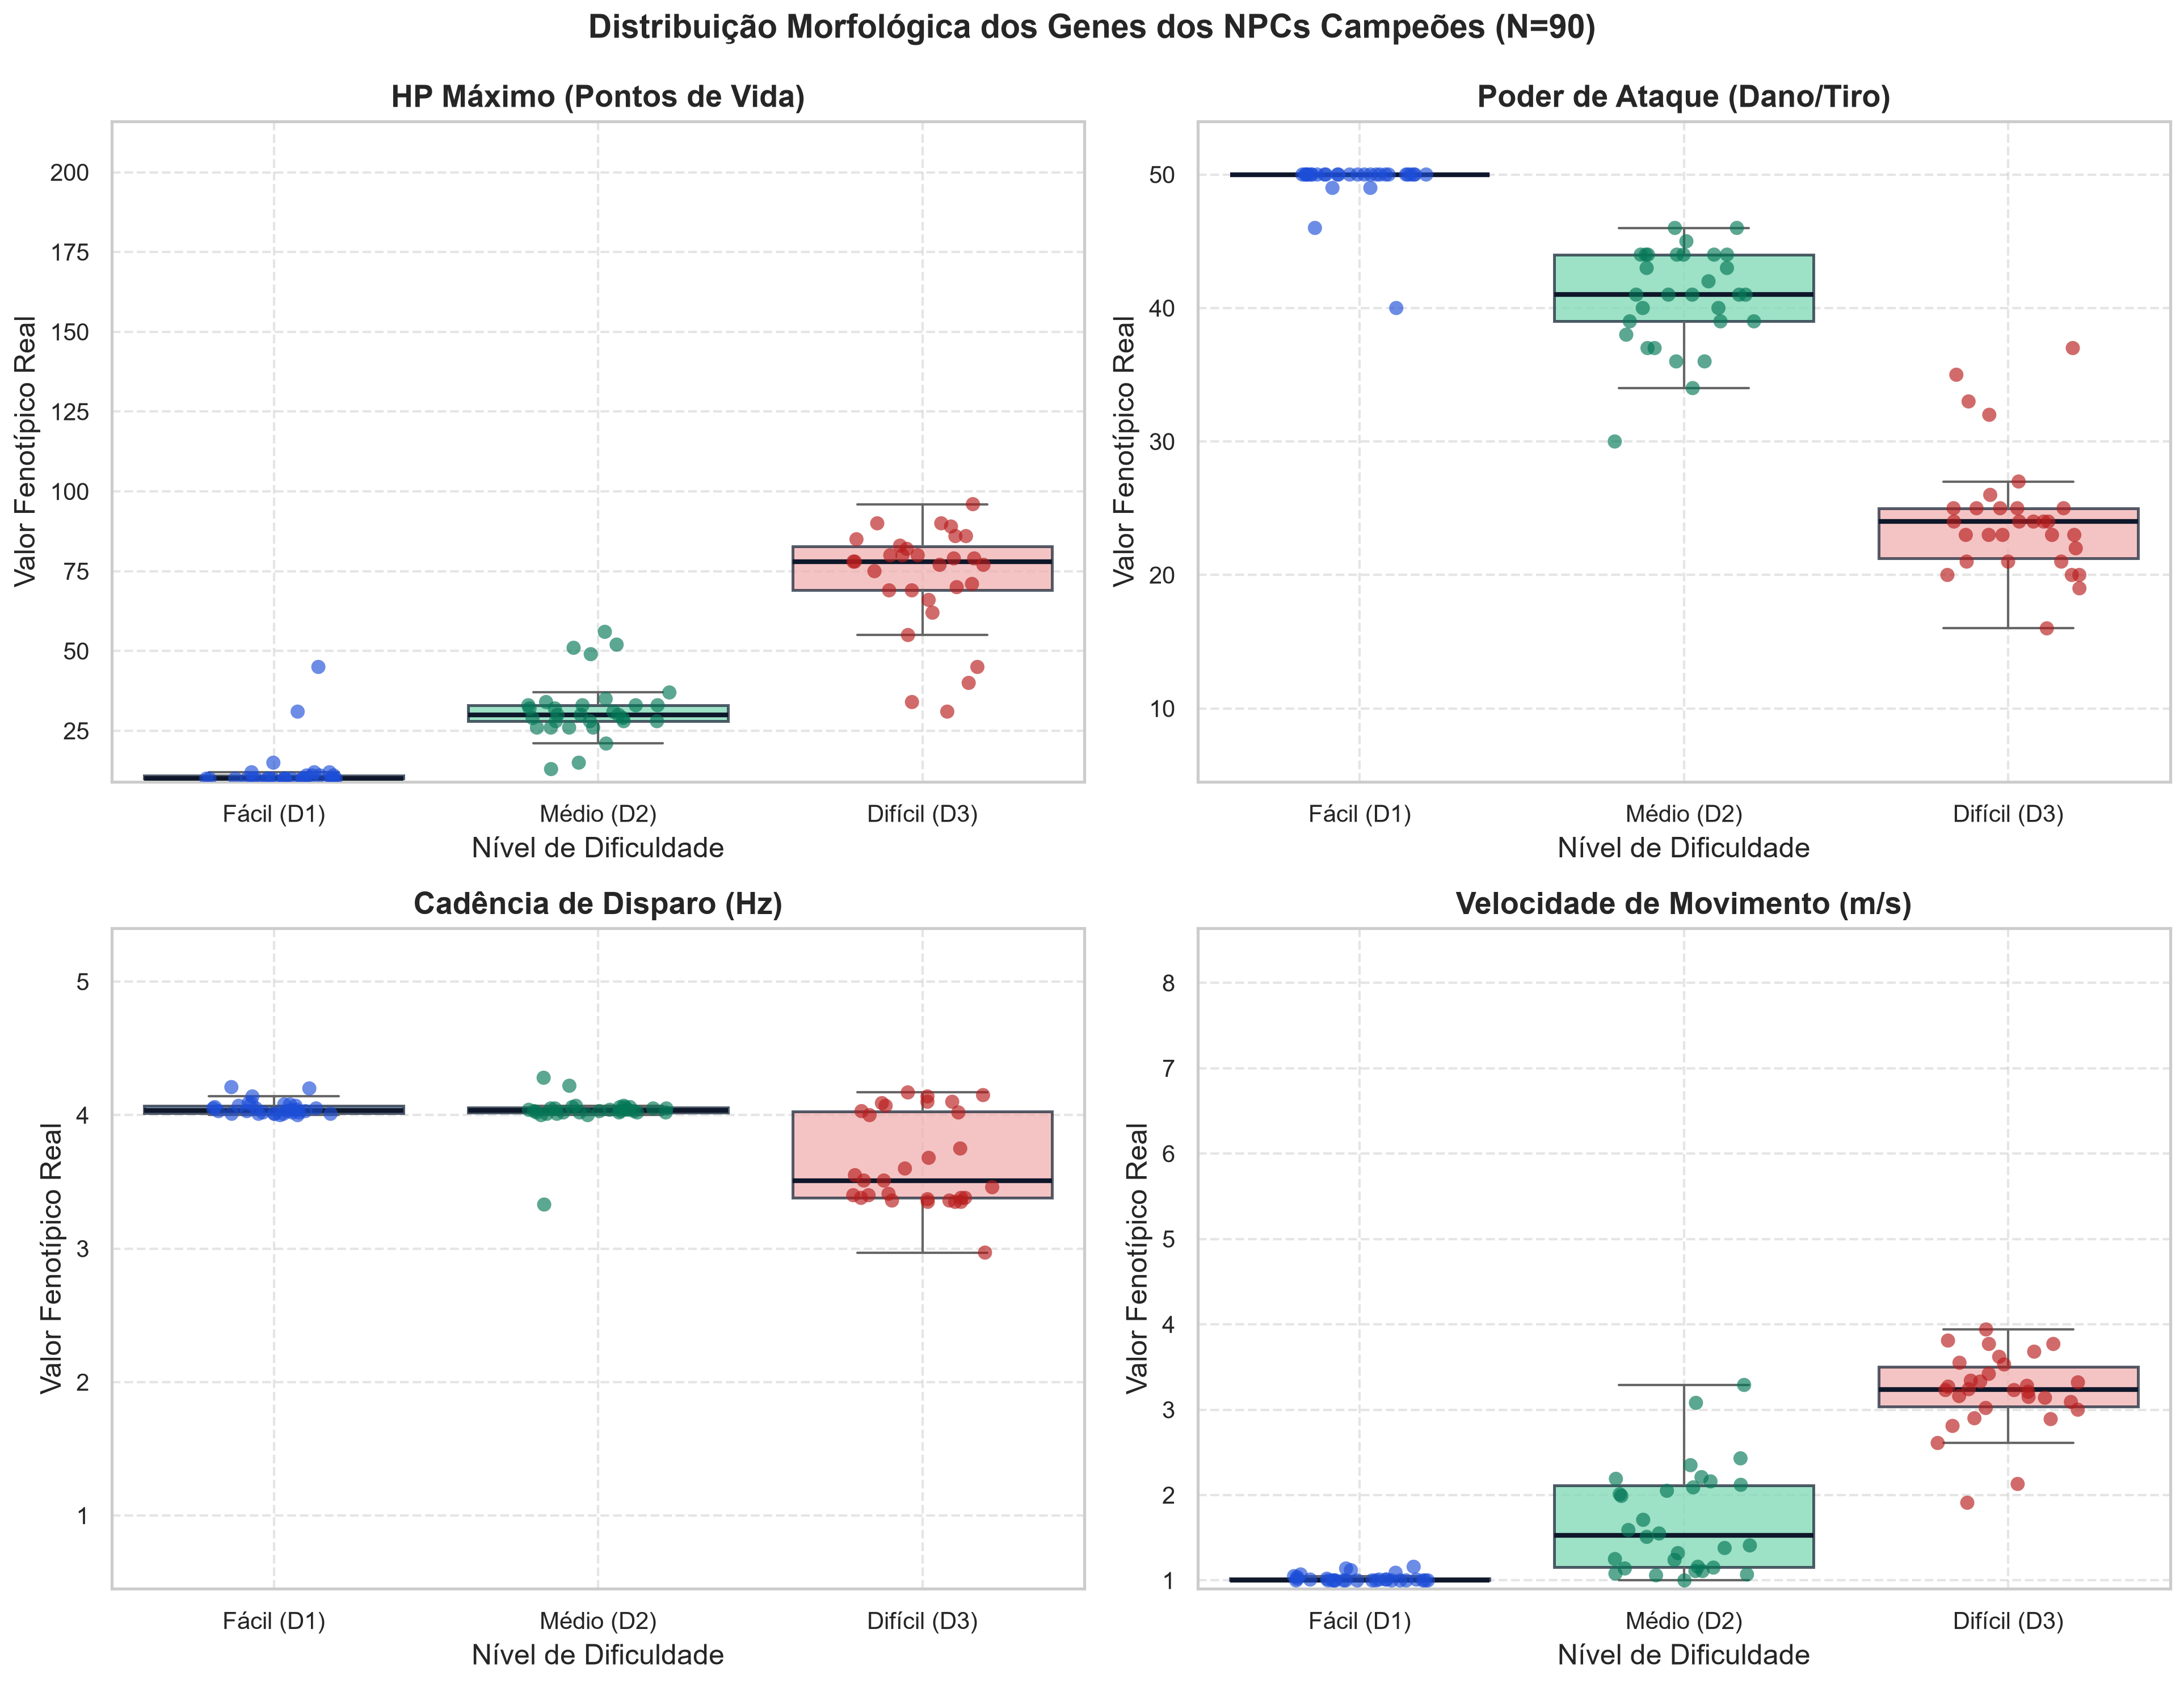
\includegraphics[width=\linewidth]{figuras/boxplot_distribuicao_genes.png}
  \caption{Dispersão dos genes fenotípicos por regime.}
  \label{fig:boxplot_genes}
\end{subfigure}
\caption{Validação estatística da separabilidade comportamental e especialização gênica sob restrição ($N = 86$).}
\label{fig:boxplots_combinados}
\end{figure*}

Emergem três arquétipos bem-definidos:
\begin{enumerate}
    \item \textbf{Tanque / Bruiser (Fácil):} $u_{\text{hp}} \approx 0{,}78$, $u_{\text{atk}} \approx 0{,}62$, $u_{\text{vel}} \approx 0{,}22$. Prioriza absorção passiva e dano bruto face à lentidão dos disparos ($9{,}0\,\text{m/s}$).
    \item \textbf{Combatente Equilibrado (Médio):} Partição uniforme de recursos: $u_{\text{hp}} \approx 0{,}45$, $u_{\text{atk}} \approx 0{,}42$, $u_{\text{cad}} \approx 0{,}40$, $u_{\text{vel}} \approx 0{,}53$.
    \item \textbf{Glass Cannon / Ninja (Difícil):} $u_{\text{vel}} \approx 0{,}94$ ($7{,}6\,\text{m/s}$), $u_{\text{cad}} \approx 0{,}45$, com vida no piso viável ($u_{\text{hp}} \approx 0{,}15$), sobrevivendo exclusivamente pela manobrabilidade CPA sob bullet hell.
\end{enumerate}

\subsection{Resultados Formais de Qualidade-Diversidade (QD)}
O processamento de $643$ registros atingiu \textbf{Cobertura de 100{,}00\%} (9/9 nichos preenchidos) e \textbf{QD-Score Global de 14.040{,}85}. O fitness máximo observado foi de $2.321{,}38$ (Tanque de Mobilidade Média). O QD-Score aumentou monotonicamente com o desafio: Fácil ($3.933{,}41$), Médio ($7.263{,}83$) e Difícil ($14.040{,}85$). A Tabela~\ref{tab:matriz_map_elites} sintetiza a matriz de notas, ilustrada na Figura~\ref{fig:map_elites}.

\begin{table}[h]
\centering
\caption{Matriz de Aptidão Máxima dos Elites no MAP-Elites}
\label{tab:matriz_map_elites}
\resizebox{\columnwidth}{!}{%
\begin{tabular}{lccc}
\toprule
\textbf{Mobilidade \textbackslash{} Classe} & \textbf{Tanker} & \textbf{Balanceado} & \textbf{Glass Cannon} \\
\midrule
Lento ($< 4{,}5\,\text{m/s}$)        & $1993{,}85$ & $1813{,}53$ & $1196{,}57$ \\
Médio ($4{,}5 \text{ a } 6{,}5\,\text{m/s}$) & $2321{,}38$ & $1733{,}83$ & $1240{,}99$ \\
Rápido ($> 6{,}5\,\text{m/s}$)       & $1536{,}14$ & $1424{,}77$ & $779{,}79$ \\
\bottomrule
\end{tabular}%
}
\end{table}

\begin{figure}[h]
\centering
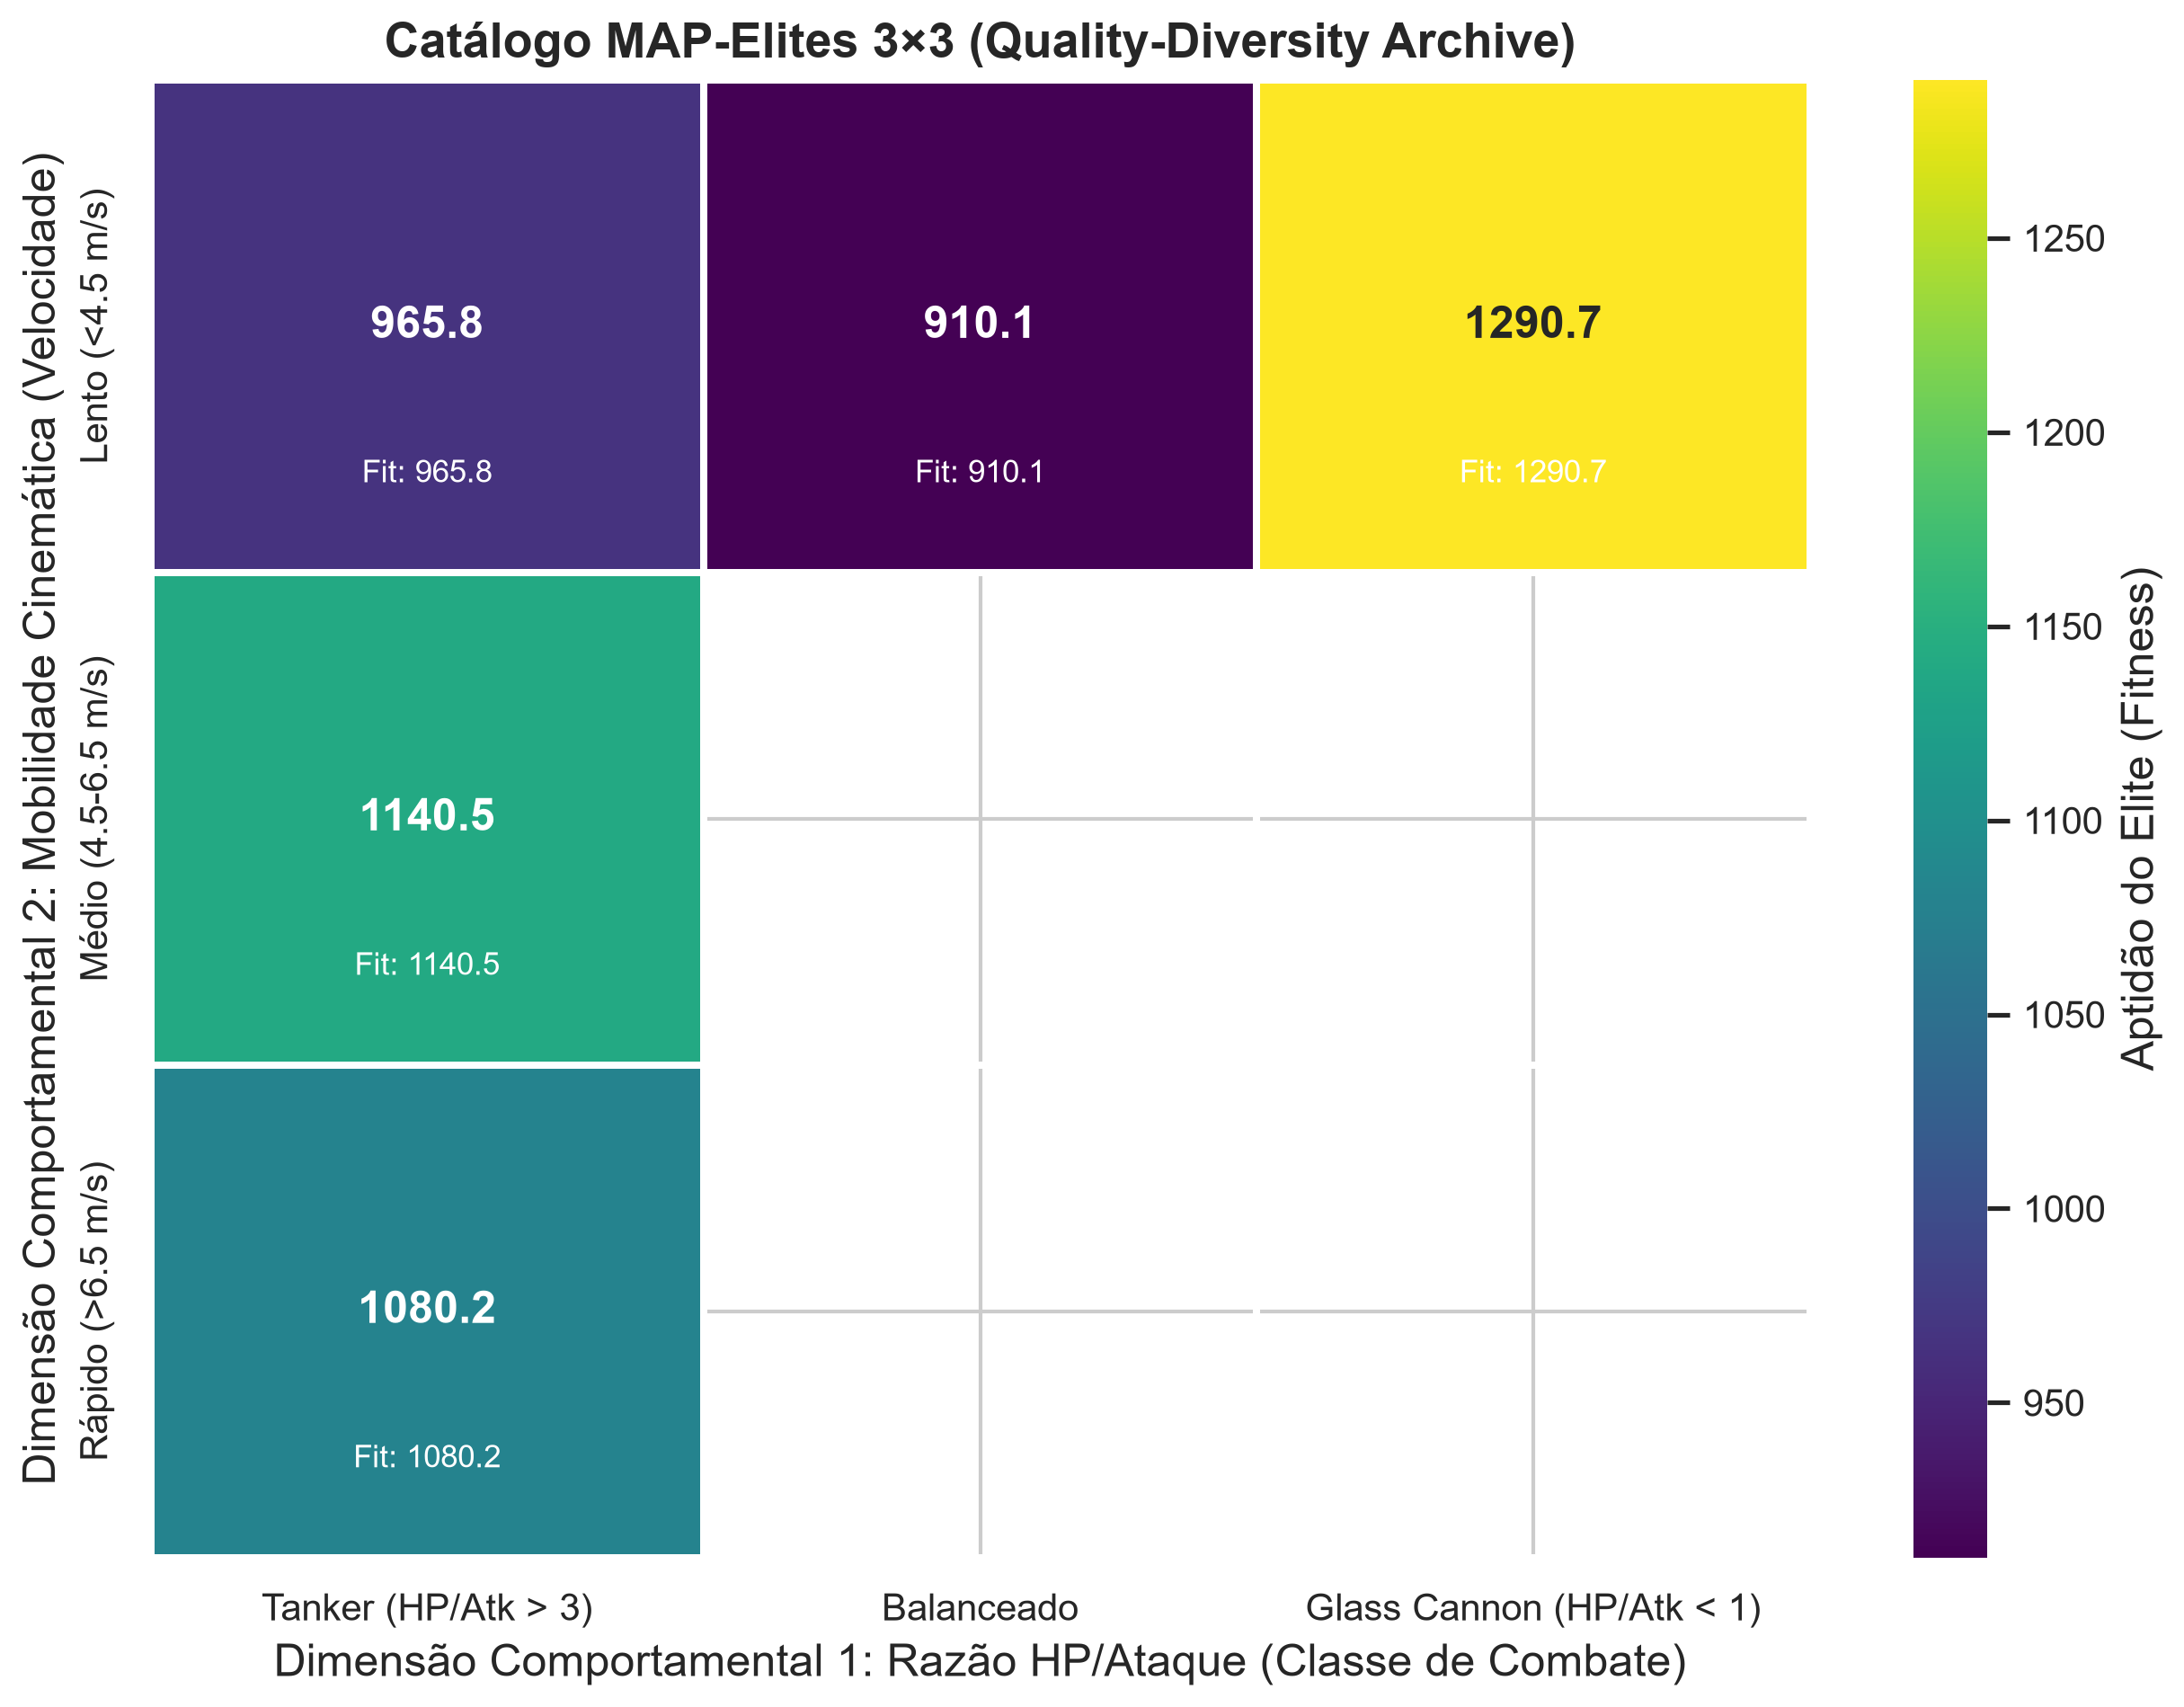
\includegraphics[width=0.88\columnwidth]{figuras/map_elites_heatmap.png}
\caption{Heatmap do MAP-Elites exibindo cobertura integral de 100\% e QD-Score consolidado de 14040.85.}
\label{fig:map_elites}
\end{figure}

\section{Estudos de Ablação}
\label{sec:ablacao}

\subsection{Ablação 1: Impacto do Orçamento \texorpdfstring{($B = 1{,}8$)}{(B = 1.8)}}
Comparou-se o Mirage padrão contra um grupo sem restrição orçamentária ($\sum u_i \le 4{,}0$). Sem o teto, $100\%$ dos indivíduos saturaram todos os genes no topo ($u_i \to 1{,}0$), colapsando a variância de velocidade para $\sigma^2_{\text{vel}} = 0{,}004$ (contra $0{,}087$ com orçamento). O sistema sucumbiu ao \textit{Reward Hacking} \cite{amodei2016concrete}, gerando agentes estáticos de $200\,\text{HP}$. Rejeita-se $H_0^{(1)}$, confirmando a necessidade do teto orçamentário para a diversidade tática (\textbf{RQ1}).

\subsection{Ablação 2: CPA e Lead-Aiming vs. Reações Puras}
Substituiu-se o CPA por repulsão reativa euclidiana proporcional e disparos sem predição balística. No modo Difícil ($D_3$), o tempo médio de sobrevivência do agente reativo foi de $11{,}40 \pm 2{,}8\,\text{s}$, contra $28{,}65 \pm 1{,}4\,\text{s}$ no agente CPA com lead-aiming ($+151{,}3\%$). A frequência de colisões críticas reduziu de $2{,}14$ para $0{,}48\,\text{hits/s}$ (redução de $77{,}5\%$, $t = 18{,}72, p < 10^{-24}$). Rejeita-se $H_0^{(2)}$, comprovando a superioridade do modelo preditivo dual (\textbf{RQ2}). A cobertura de $100\%$ no MAP-Elites atesta a catalogação contínua de elites para DDA (\textbf{RQ3}).

\section{Conclusão e Trabalhos Futuros}
\label{sec:conclusao}
O framework \textbf{Mirage} provou que a imposição de um orçamento rígido de atributos ($B = 1{,}8$) impede o \textit{Reward Hacking}, garantindo a especialização autônoma em três arquétipos funcionais. A combinação de CPA e lead-aiming analíticos assegurou superioridade cinemática decisiva. A validação empírica em $N = 86$ rodadas (ANOVA $F = 327{,}46, p < 10^{-15}$, Cohen $d > 4{,}0$) e cobertura QD de $100\%$ (QD-Score $= 14.040{,}85$) fornece solidez ao framework. Trabalhos futuros contemplarão controladores neuroevolutivos via NEAT \cite{stanley2002evolving} e testes empíricos de DDA com jogadores humanos.

\clearpage

\bibliographystyle{plain}
\bibliography{referencias}

\end{document}